% Number 550
% UFPM SFriction Algebra Units CAPMA KFriction
% Block held up to vertical cart by acceleration/friction
% KO/JG

% Watermark
\AddToShipoutPicture*{\BackgroundPic}

\addtocounter {ProbNum} {1}

\begin{floatingfigure}[r]{.2\textwidth}
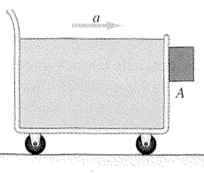
\includegraphics[scale=.6]{/Users/jgates/desktop/latex/pics/cartstatic}
\end{floatingfigure}
 
{\bf \Large{\arabic{ProbNum}}} The cart accelerates to the right, keeping block A from sliding down. The coefficient of static friction between the block and the cart is .8, and the coefficient of kinetic friction is .5. The block is 1.2 meters above the ground.

\bigskip
What minimum acceleration must the cart have in order that block A does not fall? 

\vfill
If the acceleration of the cart were only half that value, how long would it take for the block to hit the ground?
%\hfill 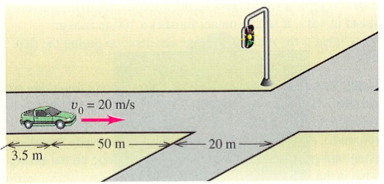
\includegraphics[scale=.85]{/Users/jgates/desktop/latex/pics/redlight.png}

\vfill
\vfill
\newpage
